\section*{Hydrogen orbitals from task 1}

\begin{figure}[!htb]
	\centering
	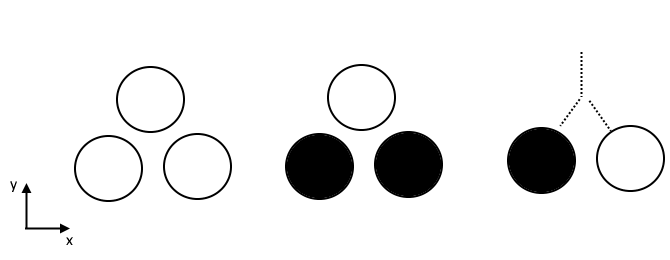
\includegraphics[width = 15cm]{Figurer/h3.png}
\end{figure}


\newpage


\section*{Task 2}

\subsection*{a)}

A Walsh diagram describes how the energy levels of a MO-diagram changes as the bonding angle changes, similarly to how the MO-diagram for octahedral complexes changes when tetragonally stretched. Such a diagram would for example describe the differences between the MO-diagrams for beryllium hydride and water or for borane and ammonia.


\subsection{b)}

\begin{figure}[!htb]
	\centering
	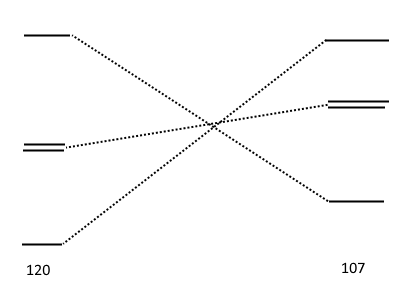
\includegraphics[width = 10cm]{Figurer/walsh.png}
\end{figure}

For \chemfig{AH_3} walsh diagrams the most bonding orbital becomes more non-bonding and the non-bonding one becomes more bonding. This is because the 2\chemfig{P_z} orbital bonds with the hydrogen group and the 2S orbital loses a lot of the bonding as the hydrogens move down below the plane. The doubly degenerated orbitals will raise slightly in energy as the hydrogen group moves out of the plane in which the 2\chemfig{P_x} and 2\chemfig{P_y} lie in and therefore both have worse overlap for bonding and start to repell each other as they get closer together.

